% !TEX root = template.tex

\begin{table*}[t]
	\begin{center}
		\begin{tabular}{ p{7cm}p{2cm}p{2cm}p{2cm}p{2cm} }
			\hline
			Method & Accuracy & Precision & Recall & F1-Score \\
			\hline
			CNN + No centering & 77.0 & 78.0 & 75.8 & 76.8 \\
			CNN + No centering + Manual F. & 75.6 & 76.8 & 73.9 & 75.3 \\
			CNN + Centering + Manual F. & 86.2 & 86.9 & 70.2 & 77.6 \\
			\textbf{CNN + Centering + Encoder F.} & \textbf{89.2} & \textbf{88.9} &  \textbf{86.1} & \textbf{86.1} \\
			\hline
		\end{tabular}
		\caption{\label{tab:model-performance} HD classification results with different featueres CNN augumentation and data preprocessing. The tests are made with our CNN with OIT, Data centering, 196 (1x16) filters, max-pool (1x4), 64 fully connected neurons, l2-regularization of $5e^{-5}$ and Adam learning rate of $2e^{-5}$.}
	\end{center}
\end{table*}

\section{Results}
\label{sec:results}

In this section we will present how we selected the appropriate hyper
parameters for the final proposed architecture presented in
Sec. \ref{sec:learning-framework}. Then we will see how some of the
preprocessing blocks and encoder or manual extracted features affect
performance onto the HD. We will also show results
for the proposed architecture with OIT applied on OD.

\subsection{Heterogenity Dataset (HD)}

In this section we evaluate performance between previous work and
different model architectures and the influences of some of the
preprocessing techniques applied. Similar to what was done in
\cite{ignatov2018real}, we carried out from the HD dataset some
representative users to test the model and then use the remaining ones
to train the model. In this case we selected users \textit{a} and
\textit{b} since we found that they are very representative among all
others. In fact models tend to be less precise with user \textit{a}
and more accurate with user \textit{b}. This mainly depends on the
user's style in walking, doing stairs and so on. In this way we are
able to compare results with other works that usually tend to evaluate
performances on unseen user.

In this training and test set settings, we evaluate the best
hyperparameters for the proposed architecture model excluding OIT
preprocessing block, since this dataset was collected with a fixed
orientation. The rest of preprocessing techniques are enabled, if not
specified.

\textbf{Autoencoder.}  In order to search for best autoencoder model
we tune hyper-parameters with grid search technique. Results are
reported in Tab. \ref{tab:ae-hyperparams} where values that performs
well on the validation dataset are reported in bold.  The best model
used to be the one with a relatively small code size: from 24 to 36
features which is also a good thing as we do not want the autoencoder
to learn the identity, but only to keep useful information.
\begin{table}[H]
  \centering
  \begin{tabular}{lp{4cm}}
    \hline
    Hyperparameter & Values \\
    \hline
    code size & \{2, 3, 4, 5, 6, 12, 18, 24, 30, \textbf{36}, 42, 48, 54, 60, 72\} \\
    batch size & \{32, \textbf{128}\} \\
    epochs & \{\textbf{150}, 200\} \\
    \hline
  \end{tabular}
  \caption{Grid-search for best hyperparameters on autoencoder}
  \label{tab:ae-hyperparams}
\end{table}

Another interesting result is, as the Tab.~\ref{tab:ae-loss} confirms,
that OIT is a necessary
operation when dealing with HAR signals. For example, without OIT we
can see that the autoencoder trained and tested on same data goes from
$0.747241$ to $10.421337$ MSE: more than $10$x worse TODO siamo in etherogenity non va bene sta comparativa qui. Furthermore,
data from hand or pocket-up/down do not inflate the loss too
much. This is good because it indicates that autoencoder is producing
robust features.
\begin{table}[H]
  \centering
  \begin{tabular}{lr}
    \hline
    Scenario & Loss (MSE) \\
    \hline
    HD + OIT + OD validation & 0.747241 \\
    HD + OIT + OD validation (allpos) & 0.821241 \\
    HD & 0.871255 \\
    HD + OD validation & 10.421337 \\
    \hline
  \end{tabular}
  \caption{Autoencoder loss on different scenarios}
  \label{tab:ae-loss}
\end{table}

Also, for checking autoencoder results we fine-tuned KNN parameters
with a grid search, looking for best values of distance measure and
number of neighbors. The Tab. \ref{tab:knn-grid-search} show the values.
We select the euclidean distance measure and $5$ as number of neighbors.
Due to time reasons we do not investigate further the FFNN model instead.
\begin{table}[H]
  \centering
  \begin{tabular}{p{2cm}p{4.5cm}}
    \hline
    Hyperparameters & Values \\
    \hline
    Distance measure & \{\textbf{euclidean}, manhattan, chebyshev, minkowski, standardized euclidean, mahalanobis\} \\
    Number of neighbors & \{3, 4, \textbf{5}, 6, 7, 8\} \\
    \hline
  \end{tabular}
  \caption{Grid-search for KNN classifier}
  \label{tab:knn-grid-search}
\end{table}

From the grid-search on KNN we suprisingly noticed that performances
do not vary so much on different hyper-parameters: we get from
$76.7$\% to $80.9$\% accuracy. This may be an indication of the
maximum capability of this autoencoder model, so to obtain better
performances we have to add complexity to the model. In particular, we
noticed that KNN usually misclassifies \textit{bike} activity with
\textit{no activity}, in fact \textit{bike} has only
$68$\% precision.

The Tab. \ref{tab:ae-classifiers-accuracy} shows KNN and FFNN accuracy
for the selected autoencoder with $36$ features and the two classifier
described in Sec. \ref{subsec:autoencoder} with hyperparameters
discussed above. Again, we can see how the OIT is really helpful in
our task: without it we couldn't event reach coin-flip
accuracy. Moreover we can say that the two models are higly correlated
in performaces with a difference of $\approx 10$\% accuracy from KNN
to FFNN. The FFNN performs better than KNN only on \textit{HD} without
OIT, but this could be due to overfitting.

\begin{table}[H]
  \centering
  \begin{tabular}{p{4cm}rr}
    \hline
    Scenario & KNN acc. & FFNN acc. \\
    \hline
    HD + OIT + OD validation & 82.2  & 72.3 \\
    HD + OIT + OD validation (allpos) &  78.9 & 68.0 \\
    HD & 76.2 & 81.8 \\
    HD + OD validation & 27.8 & 10.3 \\
    \hline
  \end{tabular}
  \caption{KNN and FFNN accuracy comparison}
  \label{tab:ae-classifiers-accuracy}
\end{table}

\textbf{CNN Network.} We fist test how number of convolutional filters and number of dense neurons in the FC2 layer will influence classification performances. The results obtained are presented in Tab. \ref{tab:model-selection}. Wee decided to choose 196 convolutional filters and 64 dense neurons thanks to its balance between accuracy and F1-Score performances, obtaining 88.9\% and 81.6\% respectively. To compare our result with that obtained in the original work \cite{stisen2015smart}, we decided to perform their \textit{Leave-one-user-out cross validation} evaluation, consisting of test the model with data from one user, and train with data from all the others in a cross validation fashion and then averaging the metrics obtained. In this evaluation setting we obtained an average F1-score of 85.8\%, beating their best model result of nearly 10\% more in F1-Score metric. This prove also that using users a and b to do our evaluation is a good compromise of the real \textit{Leave-one-user-out cross validation} evaluation performances, since we obtain nearly the same results (90.2\% instead of 88.9\% in accuracy and 85.8\% instead of 81.6\%).

\begin{table}[h]
	\begin{center}
		\begin{tabular}{ p{1.8cm}p{1.7cm}p{1.7cm}p{1.7cm} }
			\hline
			CNN Filters & Dense Neurons & Accuracy & F1-Score \\
			\hline
			196 & 1024 & 84.6 & 75.3 \\
			196 & 512 & 86.1 & 75.7 \\
			\textbf{196} & \textbf{64} & \textbf{88.9} & \textbf{81.6} \\
			96 & 1024 & 82.8 & 69.9 \\
			96 & 512 & 84.4 & 73.7 \\
			96 & 64 & 89.0 & 73.0 \\
			48 & 1024 & 80.0 & 79.4 \\
			48 & 512 & 83.7 & 74.9 \\
			48 & 64 & 84.0 & 72.3 \\
			\hline
		\end{tabular}
		\caption{\label{tab:model-selection} HD classification results with data centering and manual features augmented CNN}
	\end{center}
\end{table}


To better appreciate how our preprocessing blocks affects model overall performances, we also try to disable or enable some of them. In Tab. \ref{tab:model-performance} we report our obtained results experiments. We see that augmenting the CNN with manual extracted feature when data are not centered, lead to no significant change in performances, instead when also enabling data centering preprocessing with manual features augmented CNN the model obtain nearly 10\% more in accuracy and precision metrics. This prove the benefits of data centering stated previously. However we were not able to get the same performances obtained in \cite{ignatov2018real}, where the authors obtained in the same exact setting an accuracy of 97.6\%. These empirically confirm that performances of state-of-the-art models trained with one type of sensors are worse when dealing with smartphone sensors heterogeneity. Moving on, augmenting the CNN with encoder feature lead the model to better performances, meaning that encoder feature are more robust that manual feature, as explained previously. A confusion matrix in this latter setting is reported in Fig. \ref{fig:cnn-confusion-matrix} where we could see that the model perform nicely overall in all the considered activities, with some difficulties in distinguishing between stationary activities, stand and sit, and walk with stairs activities since that are very similar in sensor signals foot-prints.

\begin{figure}[h]
	\centering
	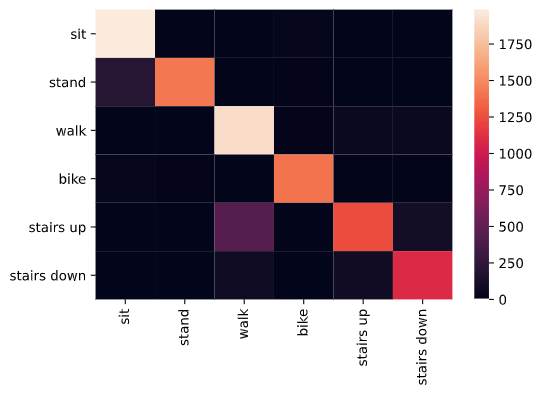
\includegraphics[width=0.5\textwidth]{images/confusion_matrix.png}
	\caption{CNN confusion matrix}
	\label{fig:cnn-confusion-matrix}
\end{figure}


\subsection{Oriented Dataset (OD)}

With these new collected dataset we want to test our model performances in a real use case scenario, where smartphone could be placed in different positions and orientations. In this case we trained the model with the entire HD as training set, and then use the OD as validation set. The Tab. \ref{tab:model-oit-performance} shows the results obtained in that configuration. We obtained great performance, in activities done holding the smarthphone in a pouch, like the ones observed in training set, even if smartphone were hold in new orientations. This mean that OIT is extremely useful preprocessing technique.
Holding smartphone in new unseen positions, like in hand or in pocket trousers, reveal some drop in model performances of nearly 15\% less. However we are pretty satisfied considering the new problem setting.
We also try to evaluate the amount of contribution of OIT preprocessing technique, by testing the model in pouch position without applying OIT. In this case, we obtain a drop of nearly 45\% in all the metrics considered, with respect to the results obtain in pouch position with OIT reported in Tab. \ref{tab:model-oit-performance}.

\begin{table}[ht]
  \begin{center}
    \begin{tabular}{p{1.8cm}rrrr}
      \hline
      Positions & Accuracy & Precision & Recall & F1-score \\
      \hline
      Pouch & 85.3 & 92.0 & 73.8 & 81.9 \\
      Hand+Pocket & 70.5 & 79.5 & 63.0 & 70.2 \\
      All & 78.0 & 84.0 & 69.0 & 75.7 \\
      \hline
    \end{tabular}
    \caption{Classification comparisons onto \textit{OD} between
      smartphone positions (pouch left/right/top/back, hand and
      pocket-up/down and all positions).}
    \label{tab:model-oit-performance}
  \end{center}
\end{table}


